%\documentclass[a4paper]{article}
\documentclass{article}
\usepackage{luatexja}                              % lualatex の場合
\usepackage[hiragino-pron]{luatexja-preset}        % ヒラギノフォント
%
\usepackage[top=3cm, left=2cm, bottom=2cm, right=2cm]{geometry}
\usepackage{fancyhdr}
\fancyhead{}
%\fancyhead[L]{\sffamily 2019/11/09}
\fancyhead[C]{\sffamily オペレーティングシステム 後半(第10回)}
\fancyhead[R]{\sffamily p.\thepage}
\fancyfoot{}
\fancyfoot[C]{} % none
\usepackage{pdfpages}

\begin{document}
%\includepdf[pages=1-last,nup=2x4,landscape=false,frame=true,
%        pagecommand={\thispagestyle{fancy}},
%        noautoscale=true,scale=0.6,delta=5mm 8mm]{mogi.pdf}
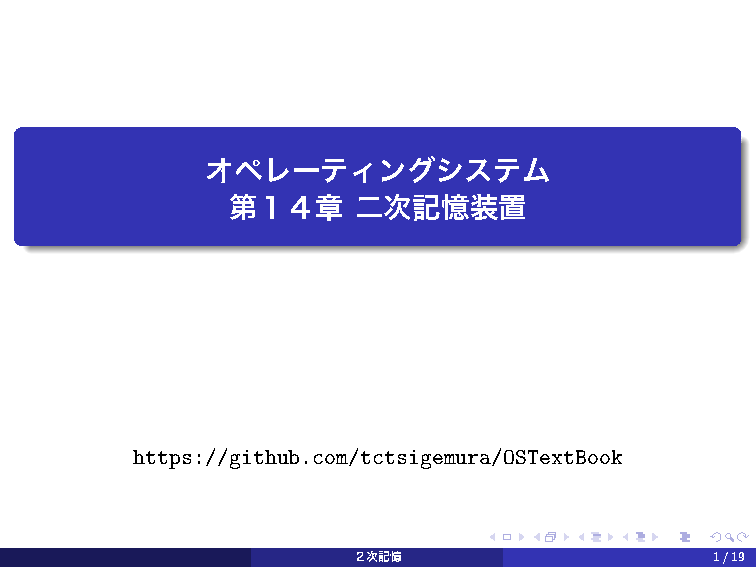
\includepdf[pages=-, %pages={1-8,10-last},
  nup=2x3,landscape=false,frame=true,
  pagecommand={\thispagestyle{fancy}},
  noautoscale=true,scale=0.65,delta=8mm 20mm]{chapE_Sld.pdf}
\end{document}
